\documentclass[conference,compsoc, twocolumn]{IEEEtran}
\ifCLASSOPTIONcompsoc
  \usepackage[nocompress]{cite}
\else
  \usepackage{cite}
\fi
\ifCLASSINFOpdf
\else
\fi
  \usepackage{amsmath} 
  \usepackage{array}
  \usepackage{fixltx2e}
  \usepackage{stfloats}
  \usepackage{url}
  \usepackage{graphicx}
\hyphenation{data-base}

\begin{document}

\title{Baseball-AI\\ Simultaneous Winning Rate Computing}

\author{\IEEEauthorblockN{Ji Am Chung\IEEEauthorrefmark{1},
Young Jae Byun\IEEEauthorrefmark{2},
Seung Myeon Park\IEEEauthorrefmark{3}, 
Jun Jeon\IEEEauthorrefmark{4}}
\IEEEauthorblockA{\IEEEauthorrefmark{1}Department of Information System\\
Hanyang University\\
Goyang, Gyeonggi Province\\ Email: hummernk@gmail.com}
\IEEEauthorblockA{\IEEEauthorrefmark{2}Department of Information System\\
Hanyang University\\
Goyang, Gyeonggi Province\\ Email: qusdudwowo@gmail.com}
\IEEEauthorblockA{\IEEEauthorrefmark{3}Department of Information System\\
Hanyang University\\
Yongin, Gyeonggi Province\\ Email: antimoto@nate.com}
\IEEEauthorblockA{\IEEEauthorrefmark{4}Department of Information System\\
Hanyang University\\
Seoul, Korea\\ Email: jeonjun2@gmail.com}}

\maketitle

\begin{abstract}
\quad Today baseball is becoming more and more popular and getting new fans. Those who just have put their first step into baseball - find it hard to follow the rules and to understand the changes in the situation. Unlike our baseball league KBO, MLB already has many meaningful methods for in-game analyzing with real time statistics. So we are going to adopt those ideas into KBO league. Winning Probability Added, which is also known as WPA, is one of good factors which allows easy understanding of the situation and the impacts that pitcher or batter makes each time. Our project aims to show ‘Winning Rate’ and ‘WPA factor’ in real-time, with the algorithm that fits KBO situation.
\end{abstract}
% no keywords


\section{Introduction}
% no \IEEEPARstart
\quad Baseball, even though the myriad scandals, attracts more and more fans and is becoming more nationwide sports. There is a major  problem that, though baseball fans are inflowing, it’s hard for beginners to understand the rules and catch situation of the match. Though baseball is much more a number-oriented sport than any others such as soccer or basketball, the classical stats do not fully reflect the match stream and evaluate the value of the players properly. However, in MLB, a lot of sabermetricians have already quantified vague situations and values in numerical way, and KBO tends to follow it. (i.e Babip, OPS, etc..). Korean baseball websites nowadays use the same WPA algorithm which had been used in earlier days of MLB, so the differences between two leagues are not considered. We wanted to solve this problem by creating our own WPA algorithm based on KBO, which not only calculates the stats suitable for KBO, but also analyzes winning possibilities of each team and the impacts each players make. We also focus on helping beginners to understand baseball.
\quad We will make KBO winning rate DB and we are going to put that into our program. The program  represents ongoing situation of the match and each team’s winning possibilities simultaneously. Also, by showing quantified stats such as batters’ WPA or pitchers’ WAR , it shows how much powerful the player is(or has been) throughout the game, seasons or his entire career. Whether baseball match is underway or not, the program will show player rank categorized by players, teams, or positions according to user’s request.
\quad It is not just ‘Baseball statistic calculator’, but also somewhat like websites such as Statiz or KBReport. The software indicates different types of statistical analysis, and shows them in visualized ways. We thought that current WPA algorithm used in korean web sites does not fit korean baseball situation. That is why we have started this project.

This project is composed of 4 steps.
\begin{enumerate}
\item Crawl the data of  last 10 seasons of KBO from baseball statistics websites. 
\item Compute the data to make some statistics.
\item Apply the statistics to WPA algorithm.
\item Real-time data capturing and showing the winning rate and WPA.
\end{enumerate}
% You must have at least 2 lines in the paragraph with the drop letter
% (should never be an issue)

\hfill May 2, 2016



\section{Requirements}



\subsection{Data Handling}


\subsubsection{Crawling}
\begin{itemize}
\item Get every single raw data of  KBO from baseball webpage to construct the root database.
\item Crawiling source : http://www.koreabaseball.com
\end{itemize}

\subsubsection{Capturing}
\begin{itemize}
\item Get real-time data when the match is underway.
\end{itemize}

\subsubsection{Real-Time Mirroring}
\begin{itemize}
\item Program should immediately renew the database according to the result of the match.
\end{itemize}

\subsubsection{Computing}
\begin{itemize}
\item Calculate the numerical data to make some meaningful statistics.
\item Every single data has different weight.
e.g.)\ Hits at 1st inning have different value from those at 9th.
\item Calculate numerical values including WPA.
\end{itemize}

\subsubsection{Data Storage}
\begin{itemize}
\item Save every single stats data.
\item Divide players  into two tables. One table is for players who is in active service, the other for retired.
\item Table for players who is in active service needs to be updated constantly, and the other table doesn’t.
\item User who wants to conceal  the program from screen can do that by clicking ‘window minimization’ button.
\end{itemize}

\subsection{Function}


\subsubsection{EXCEL Compatibility}
\begin{itemize}
\item User can export datas of specific player or stats  to MS Excel files.
\item User can import fixed form of MS Excel file of specific game result to compute changes of KBO algorithm winning rate shown as image file which can also exported as jpeg, gif, png, or bmp.
\item User can import fixed form of MS Excel file of specific league(fantasy or amatuer) data to compute WAR stats. This data can be exported as EXCEL file.
\end{itemize}

\subsubsection{On-Board Posting(abandoned)}
\begin{itemize}
\item Someone who wants to post any idea or thoughts can share what they have.
\item Make another Q\&A board so as to hel beginners solve their curiosity.
\end{itemize}

\subsubsection{Board Log-in \& Sign-out(abandoned)}
\begin{itemize}
\item Log-in to or Sign-out from Board.
\item User who logged-in the board can upload their post or reply to other users’
\end{itemize}

\subsubsection{Stats Visualization}
\begin{itemize}
\item Show current state of game in a table.
\item Show current winning average of each team 
\item Show current WPA stats of players
\item Show player's photograph
\end{itemize}

\subsection{User Interface}


\subsubsection{Window Minimization \& Window Maximization}
\begin{itemize}
\item User who wants to see the program widely can do that by clicking ‘window maximization’ button
\end{itemize}

\subsubsection{Program Turn On \& Turn Off}
\begin{itemize}
\item User can turn on the program by clicking ‘desktop icon’ 
\item If user try to power on the program even if that is already turned on, terminate existing program and launch the program again
\item User can turn off the program by clicking ‘x button’ at the top-right corner of the program
\end{itemize}

\subsubsection{Mouse Click Event}
\begin{itemize}
\item Provide user with three options [To Home, Window Minimization, Termination] when user right-click any area within program.
\end{itemize}

\subsubsection{Player Stat Pop-Up}
\begin{itemize}
\item When user clicks certain player, program shows his profile by generating a new pop-up
\item If player is a pitcher, pop up list of the first string who has not on the match yet
\item If player is taking the field, pop up his profile as batter
\item Pitcher pop-up profile stats list : ERA(Earned Run Average) for applicable season, WPA, WAR, WHIP for last 5 matches, (K\/BB 9), hyperlink connected to NAVER article about him
\item Batter pop-up profile stats list : BA(Batting Average), WAR, WPA, OPS for last 5 matches, BABIP for applicable season, \quad hyperlink connected to NAVER article about him
\item The number of pop-up cannot be over two
\end{itemize}

\subsubsection{Player Ranking}
\begin{itemize}
\item Sort players by team, position, date and game with WPA stats
\end{itemize}

\subsubsection{Data Searching}
\begin{itemize}
\item Searching option constitutes of match schedule, player and stats and player
\item If option ‘match schedule’ is chosen, program shows match schedule as a calendar
\item If user click one of date, there are three cases. First one is ‘past match’, so program shows match log. Second one is ‘on-going match’, so program directs user to the match. And the last one is ‘coming match’, so program shows every details of  the match including players, referees, park,  appointed first thrower, weather forecast 
\item If option ‘player and stat’ is chosen, program shows the applicable stats separately by entire players,  team, position, monthly
\item If option ‘player’ is chosen, program shows every single stat of applicable player
\end{itemize}

\subsubsection{Get Information real-time}
\begin{itemize}
\item User can choose the way one gets some information(pop-up or push window)
\item Pop-up is a kind of window, so when user have it on the screen, one cannot click main program
\item Information could be as follows
\item Agreed Decision : User can get information about agreed decision and its details
\item Cancellation in case of rain : User can get information when the match is cancelled in case of rain by getting a pop-up or push window
\item Player Substitute : In case of substituting player, User can get information why the player was substituted with other, and information about that ‘other’ player
\item When option is ‘pop-up’, user can have additional function which is ‘Multi-View’.  By doing so, user can watch several matches simultaneously
\item If there have multiple pop-ups, eliminate pop-up windows sequentially after checking them
\end{itemize}

\subsubsection{Error}
\begin{itemize}
\item Error alert
\end{itemize}



\section{Development Environment}



\subsection{Choice of Software Development Platform}


\subsubsection{Which platform and why? (e.g.\ , Windows, Linux, Web, or etc.\ )}
\begin{itemize}
\item We adopted Windows, because there are some merit when we choose Windows. First of all, the percentage of all Windows user is almost 85\%. Since we want to emphasize on majority, we chose Windows. Second, because of encoding compatibility. For more convenience, it’s much better to share encoding method in OS, web server, database.
\end{itemize}

\subsubsection{Which programming language and why?}
\begin{itemize}
\item There are some technical reasons why we chose programming language ‘Go’ made by google. After a long discussion that lasted several days, group members agreed to implement the program with google Go. Because, different from C or Java, we can easily reflect up-to-date version through cloud. That would help us to keep up with newest trends in software developing, so that we can always maintain the high level stability of the program.
\end{itemize}

\subsubsection{Provide a cost estimation for your built.\\
 (including any purchase of software/hardware)}
\begin{itemize}
\item human labor - 0 \\
Our group constitute of four members who all do this group term project voluntarily. So human labor cost is zero.
\item software cost - 0  \\
Our group will make program with open source API,  which costs zero for academic purpose.
\item hardware cost - 0  \\
Our group uses our existing laptop to simulate or implement our program. There is no need to buy other hardware. 
\end{itemize}

\subsubsection{Provide clear information of your development environment.\\
(e.g., version of software, OS version, your computer resources)}
\begin{itemize}
\item OS \\
Windows 10 pro(10586.218 build)
\item Language Set \\
Korean
\item Computer Mode l\\
MSI GT60
\item Processor \\
Intel(R) Core(TM) i7-3600QM	CPU @ 2.4GHz
\item Main Memory \\
8GB RAM
\item Internet Connection \\
IPTIME WiFi
\end{itemize}


\subsection{Software in use}


\subsubsection{Any existing software or algorithm in use? (doing a similar task as
your proposal; provide a proper reference if there is any)}
\begin{itemize}
\item There is no similar software computing WPA, after Tom Tango present concept of WPA.
\item Rather, there are some websites providing some information which can help users WPA by themselves.
\end{itemize}

Statiz
\begin{figure}[h]
\centering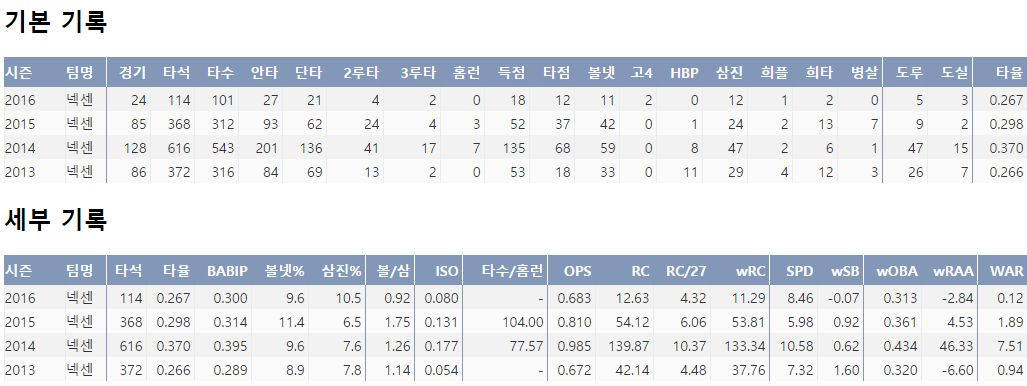
\includegraphics[width=6cm]{Statiz}     
\caption{Statiz}
\end{figure}
\\
\\
\\

KBReport
\begin{figure}[h]
\centering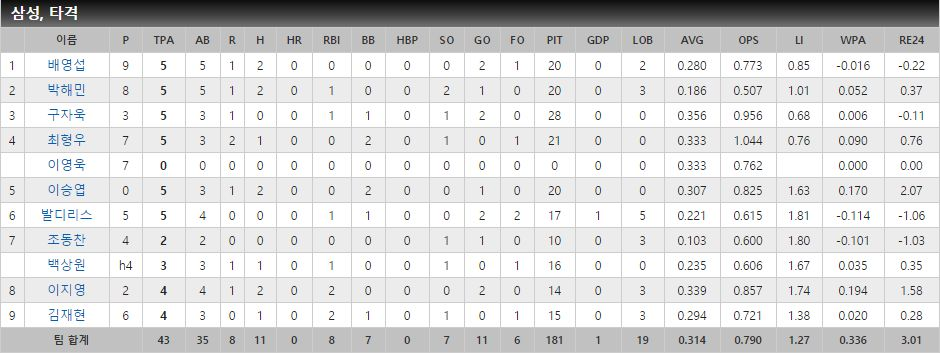
\includegraphics[width=6cm]{KBReport}    
\caption{KBReport}
\end{figure}

TheBook
\begin{figure}[h]
\centering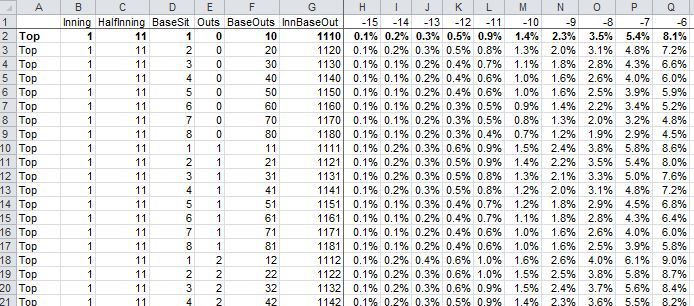
\includegraphics[width=6cm]{TheBook}
\caption{TheBook}
\end{figure}




\subsection{Task distribution (If you want, you can provide this
later at the next phase - design)}

\begin{itemize}
\item Which member is responsible for what?
\end{itemize}
\begin{center}
\begin{tabular}{1|1|1} \hline
Roles				& name 			&task description and etc.\  		\\ \hline
User     			& 				& 			 			\\ \hline
Customer      			&  				& 		 				\\ \hline
Software developer 	      	&  				&  		 				\\ \hline
Delopment manager      	&  				& 		 				\\ \hline
\end{tabular}
\end{center}



\section{Specification}


\subsection{Data Handling}

\subsubsection{Crawling}
\begin{figure}[h]
\centering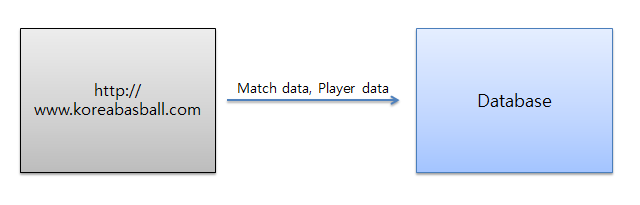
\includegraphics[width=6cm]{requirement1-a}
\caption{crawling}
\end{figure}

\begin{itemize}
\item Get every single data from baseball webpage to construct the database.
\item Data means game box score which contains every statement in actual game.
\item Crawiling source : \\
	http://www.koreabaseball.com/Schedule/Game/Box\\Score.aspx?leagueId=n\&seriesId=0\&gameId=yyyy\\mmddt1t2x\&gyear=yyyy\\
	n of leagueId is arbitrary 1 digit number, yyyymmddt1t2x of gameId is year, month, day, team1, team2, 1 digit ordinal number, yyyy of gyear is year
\item Crawler tries to crawl web data every 30 second.
\end{itemize}


\subsubsection{Capturing}
\begin{figure}[h]
\centering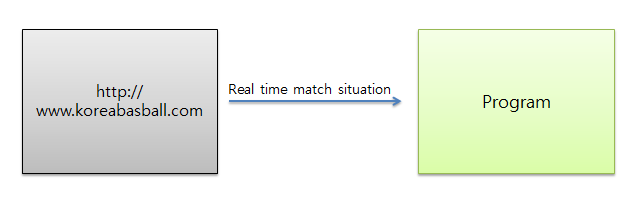
\includegraphics[width=6cm]{requirement1-b}
\caption{capturing}
\end{figure}

\begin{itemize}
\item Get real-time data when match is underway.
\end{itemize}


\subsubsection{Real-Time Mirroring}
\begin{figure}[h]
\centering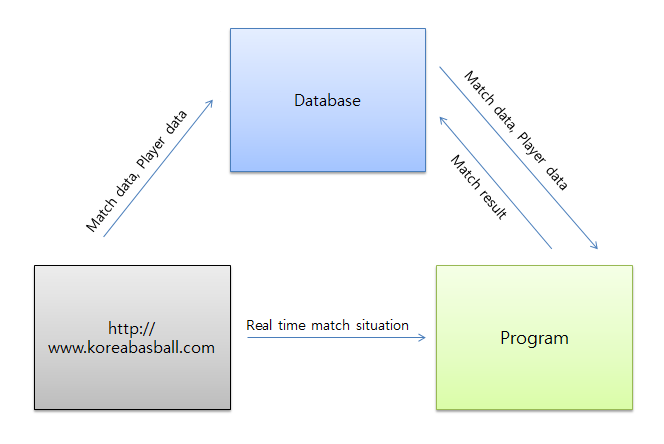
\includegraphics[width=6cm]{requirement1-c}
\caption{real-time mirroring}
\end{figure}

\begin{itemize}
\item Program should immediately renew the database according to the result of the match.
\end{itemize}


\subsubsection{Computing}
\begin{itemize}
\item \begin{equation} \label{eq:winrate} Winrate = \frac{All Matches\cap Statement\cap Win}{All Matches\cap Statement} \end{equation}
\end{itemize}



\subsubsection{Data Storage}
\begin{itemize}
\item Save every single stats data.
\item Divide players  into two tables. One table is for players who is in active service, the other for retired.
\item Table for players who is in active service needs to be updated constantly, and the other table doesn’t.
\end{itemize}



\subsection{Functions}

\subsubsection{EXCEL Compatibilty}
\begin{figure}[h]
\centering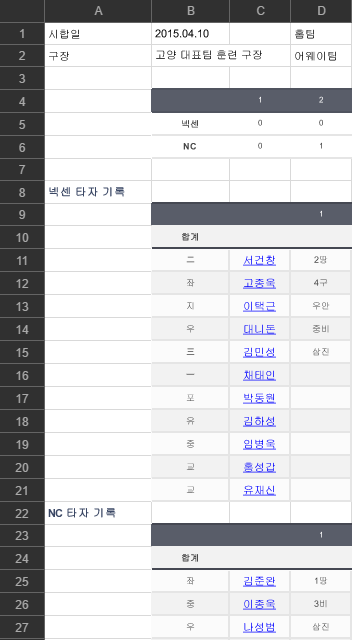
\includegraphics[width=6cm]{input}
\caption{excel input file}
\end{figure}

\begin{figure}[h]
\centering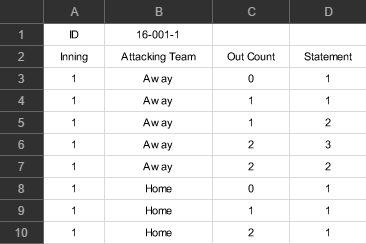
\includegraphics[width=6cm]{output}
\caption{excel output file}
\end{figure}


\begin{itemize}
\item User can export data in the program that she/he wants.
\item playerorstats.xlsl is an example of excel file daeling with datas of specific player or stats.
\item gameres.xlsl or gameres.jpeg are examples of fixed form of MS Excel file of specific game result to compute changes of KBO algorithm winning rate shown as image file which can also exported as jpeg, gif, png, or bmp.
\item leaguedata.xlsl is an example of fixed form of MS Excel file of specific league(fantasy or amatuer) data to compute WAR stats.
\end{itemize}

\subsubsection{On-Board Posting(X)}
\begin{itemize}
\item Someone who wants to post any idea or thoughts can share their idea.
\item Make another Q&A board so as to help beginners solve their curiosity.
\end{itemize}

\subsubsection{Board Log-in \& Sign-out(X)}
\begin{itemize}
\item Log-in to or Sign-out from Board.
\item User who logged-in the board can upload their post or reply to other post.
\end{itemize}

\subsubsection{Stats Visualization}
\begin{itemize}
\item cur\_state.myd is an example of mysql data file showing current state of game in a table form.
\item By Generating a new pop-up, program can show user current winning average of each team.
\item By Generating a new pop-up, program can show user current WPA stats of players.
\item By Generating a new pop-up, program can show player's photograph.
\end{itemize}



\subsection{User Interface}


\subsubsection{Window Minimization & Window Maximization}
\begin{figure}[h]
\centering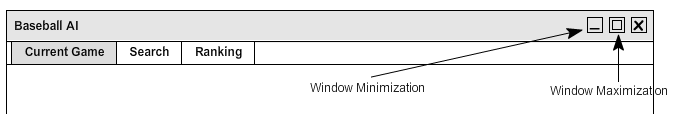
\includegraphics[width=6cm]{WindowMaxMin}
\caption{Windows Minim.\&Maxim.}
\end{figure}

\begin{itemize}
\item Window default size : 960*540
\item User who wants to conceal the program from the screen can do that by clicking ‘window minimization’ button.
\item User who wants to see the program widely can do that by clicking ‘window maximization’ button.
\item User can turn off the program by clicking ‘x button’ at the top-right corner of  the program.
\end{itemize}


\subsubsection{Program Turn On \& Turn Off}
\begin{figure}[h]
\centering\includegraphics[width=6cm]{icon}
\caption{Program Turn On}
\end{figure}

\begin{itemize}
\item User can turn on the program by clicking ‘desktop icon’.
\item If user try to power on the program even if that is already turned on, terminate existing program and launch program again.
\end{itemize}

\begin{figure}[h]
\centering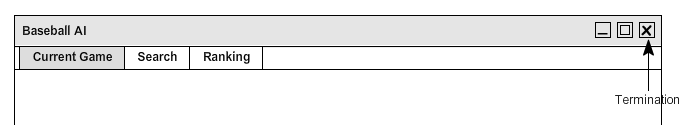
\includegraphics[width=6cm]{WindowTerminate}
\caption{Program Turn Off}
\end{figure}

\begin{itemize}
\item User can turn off the program by clicking ‘x button’ at the top-right corner of  the program.
\end{itemize}


\subsubsection{Mouse Click Event}
\begin{itemize}
\item Provide user with three options [To Home, Window Minimization, Termination] when user right-click any area within program.
\end{itemize}

\subsubsection{Player Stat pop-up}
\begin{itemize}
\item When user clicks certain player, program shows his profile by generating a new pop-up.
\item If player is a pitcher, pop up list of the first string who has not on the match yet.
\item If player is taking the field, pop up his profile as batter.
\item Pitcher pop-up profile stats list : ERA(Earned Run Average) for applicable season, WPA, WAR, WHIP for last 5 matches, (K/BB 9), hyperlink connected to NAVER article about him.
\item Batter pop-up profile stats list : BA(Batting Average), WAR, WPA, OPS for last 5 matches, BABIP for applicable season, hyperlink connected to NAVER article about him.
\item The number of pop-up cannot be over two.
\end{itemize}


\subsubsection{Current Game}
\begin{figure}[h]
\centering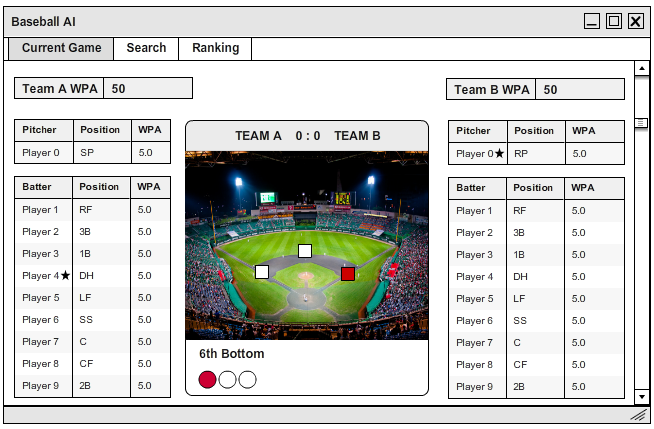
\includegraphics[width=6cm]{Current-game.png}
\caption{Current Game}
\end{figure}

\begin{itemize}
\item Star mark indicates that pitcher(player 4) is on the mound and the batter is at bat.
\item Squares on the field indicate each base. If runner is on the base, then it is colored with red.
\item Circles at the bottom of the field indicate out count. Red is counted and blank is not.
\end{itemize}


\subsubsection{Player Ranking}
\begin{figure}[h]
\centering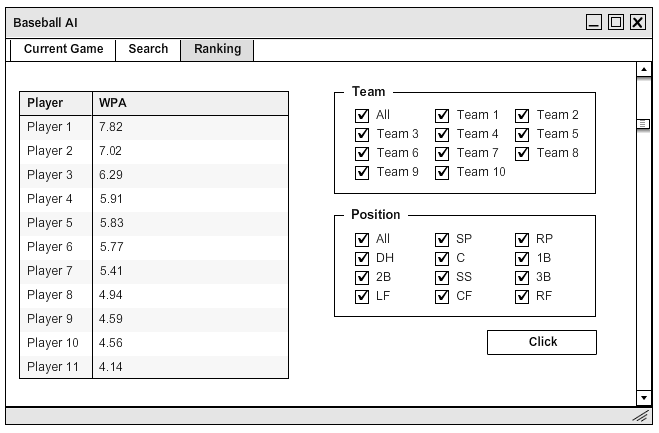
\includegraphics[width=6cm]{Ranking}
\caption{Player Ranking}
\end{figure}

\begin{itemize}
\item Sort players by team, position with WPA stats.
\end{itemize}


\subsubsection{Data Searching}
\begin{figure}[h]
\centering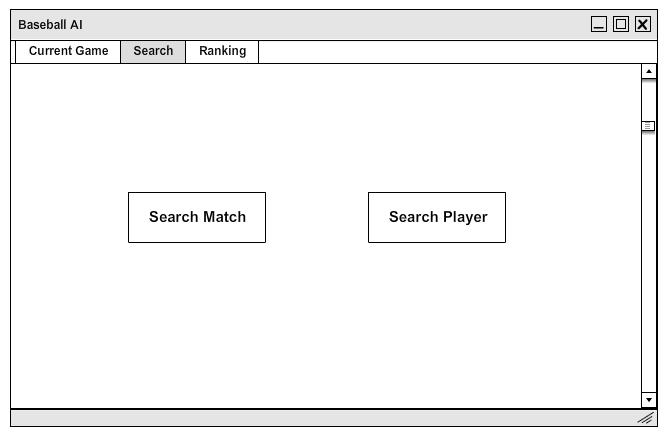
\includegraphics[width=6cm]{Search}
\caption{Search Option}
\end{figure}
\begin{itemize}
\item Search option constitutes of  ‘Search Match/ Search Player’
\end{itemize}

\begin{figure}[h]
\centering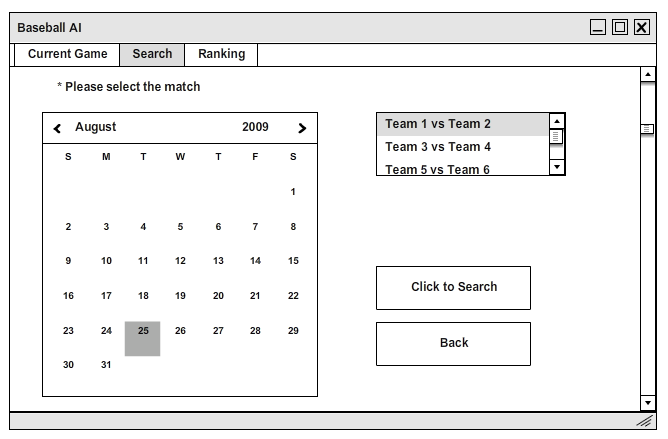
\includegraphics[width=6cm]{Search-match}
\caption{Search-match option}
\end{figure}
\begin{itemize}
\item If option ‘Search Match’ is chosen, program shows match schedule as a calendar.
\end{itemize}

\begin{figure}[h]
\centering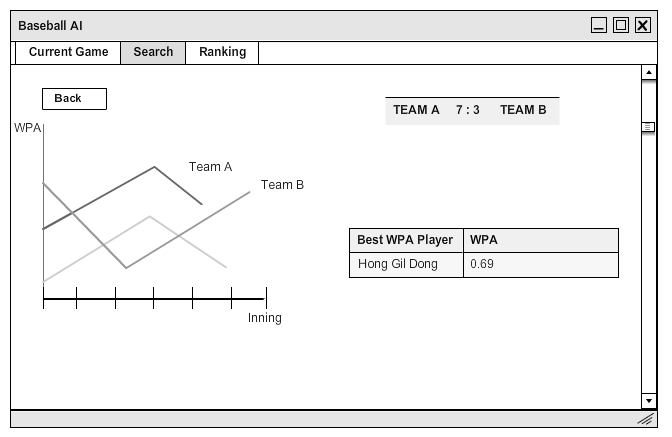
\includegraphics[width=6cm]{Search-match-result}
\caption{Search match result}
\end{figure}
\begin{itemize}
\item The result is shown above.
\end{itemize}

\begin{figure}[h]
\centering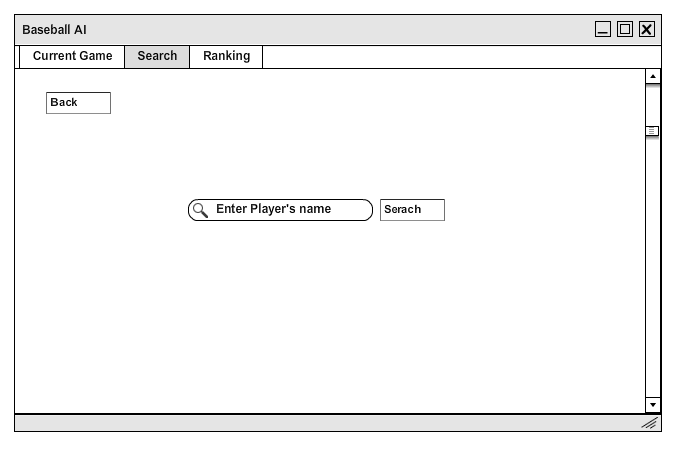
\includegraphics[width=6cm]{Search-player}
\caption{Search Player}
\end{figure}
\begin{itemize}
\item If option ‘Search Player’ is chosen, input box will appear. It requires user to enter a player’s name.
\end{itemize}

\begin{figure}[h]
\centering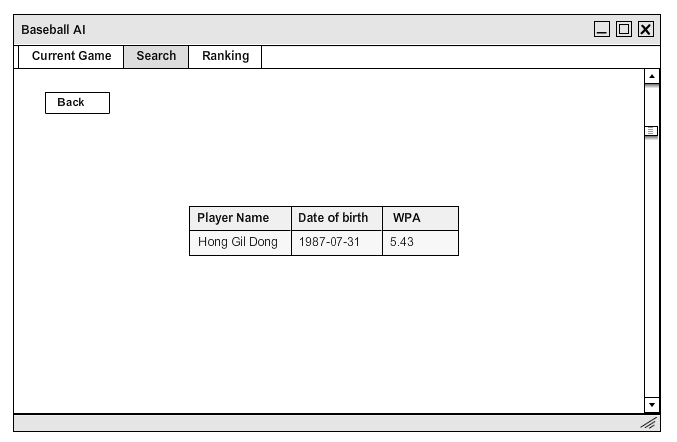
\includegraphics[width=6cm]{Search-player-result}
\caption{Search Player Result}
\end{figure}
\begin{itemize}
\item The result is shown as above.
\end{itemize}


\subsubsection{Get Information Real-Time}
\begin{itemize}
\item User can choose the way one gets some information(pop-up or push window).
\item Pop-up is a kind of window, so when user have it on the screen, one cannot click main program.
\item Information could be as follows.
\item Agreed Decision : User can get information about agreed decision and its details.
\item Cancellation in case of rain : User can get information when the match is cancelled in case of rain by getting a pop-up or push window.
\item Player Substitute : In case of substituting player, User can get information why the player was substituted with other, and information about that ‘other’  player.
\item When option is ‘pop-up’, user can have additional function which is ‘multi-view’.  By doing so, user can watch several matches simultaneously.
\item If there has multiple pop-ups, eliminate pop-up windows sequentially after checking them.
\item Refresh in every 30 seconds.
\end{itemize}



\subsubsection{Error}
\begin{figure}[h]
\centering\includegraphics[width=6cm]{error1}
\caption{Error Notification}
\end{figure}

\begin{itemize}
\item  If program does not receive signal for 2 minutes, error message pops up with alert sound(windows alert sound).
\end{itemize}

\subsubsection{Database}
\begin{itemize}
\item We need four data tables, and each every table refers to each other.
\item We also need one Season table.
\end{itemize}


\begin{figure}[htbp]
\centering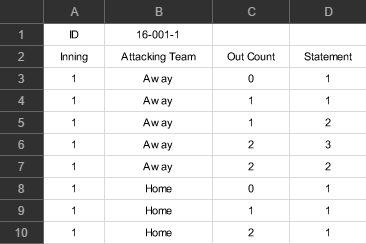
\includegraphics[width=6cm]{match_table_1}
\caption{the first half match table}
\end{figure}

\begin{figure}[htbp]
\centering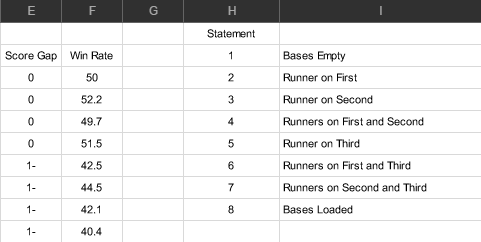
\includegraphics[width=6cm]{match_table_2}
\caption{the second half match table}
\end{figure}

\begin{figure}[htbp]
\centering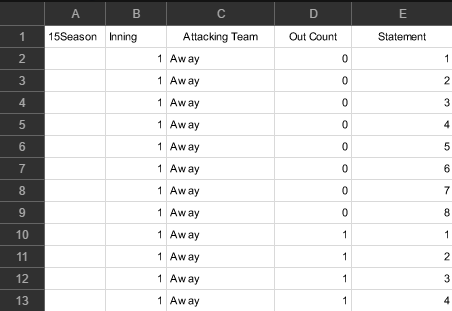
\includegraphics[width=6cm]{sea_state_1}
\caption{the first half season statement table}
\end{figure}

\begin{figure}[htbp]
\centering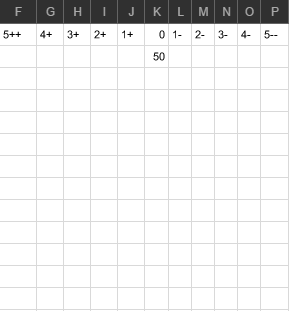
\includegraphics[width=6cm]{sea_state_2}
\caption{the second half season statement table}
\end{figure}

\begin{figure}[htbp]
\centering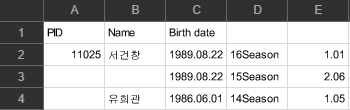
\includegraphics[width=6cm]{player_table}
\caption{player table}
\end{figure}


\section{Design}

\subsection{Design Detail}

\end{document}



















